\newpage
\setcounter{table}{0}
\setcounter{figure}{0}
\section{背景及相关工作}

\subsection{NVIDIA GPU硬件}
\subsubsection{GPU芯片总体结构} 
\par 在介绍新老架构区别之前,本节首先自顶向下简要介绍一下NVIDIA GPU芯片的结构。一块GPU芯片拥有若干图形处理器簇(Graphics Processing Cluster, GPC),由外围总线进行调度管理;一个图形处理器簇上有若干纹理处理器簇(Texture Processing Cluster, TPC);需要注意的是以上两种结构在编写CUDA程序时并不暴露。一个纹理处理器簇上有若干流多处理器单元(Stream Multiprocessor, SM),也是本文关注的重点。流多处理器单元被一个线程块调度器管理,所有流多处理器单元通过全局内存总线经过L2缓存共享全局内存。每个流多处理器单元中由若干流处理器(Stream Processpr, SP),然而这一概念随着流多处理器单元中运算单元种类的增加而被弱化了。在一个流多处理器单元内部的流处理器共享一个指令缓存,每个流处理器拥有自己的线程束调度器与寄存器文件;流处理器中包含若干种执行单元,有浮点单元,整数单元,在新架构中还加入了张量单元(Tensor Core),在RTX 2080TI上具体的参数为:一个SM包含64个单精度浮点算术单元,32个双精度浮点算术单元,64个32位整形算术单元,8个混合精度张量单元,4个线程束调度器和16个特殊功能单元;所有流处理器通过显存纵横矩阵(CrossBar)访问共享内存,或被称为L1缓存\cite{EXPLORING}。
\subparagraph{流多处理器单元(SM)} 
\par 上文提到过,六多处理器单元(SM)是本文关注的重点,其原因是每一次NVIDIA GPU芯片更新都会伴随着其计算能力(Compute Capability)的更新,计算能力指的是流多处理器单元(SM)支持的运算的等级,分为Major和Minor。其中Major代号代表架构的更新,这也会带来许多新的硬件支持的运算,而Minor代号则代表同一架构下不同定位的流多处理器产品。如伏特架构的计算能力为7.2,图灵架构的计算能力为7.5,Major代号一样就代表这两种架构其实并无太大修改,而Minor代号则代表伏特架构中流多处理器的类型是Heavy,图灵架构中流多处理器的类型是Lite。Lite和Heavy一般用于区分消费级/工作站级GPU,分别对应GeForce和Tesla代号。
\par 流多处理器单元中的不同类型的流处理器对应了不同的流水线,不同流水线的延迟、吞吐量均不同。且有些流水线指令发射是互斥的,即互斥流水线的指令不能同一时间发射,这将在下文介绍新硬件架构时提到,本文中主要关注流多处理器上的计算指令流水线(M-Pipe),光栅等其他计算涉及的流水线不做介绍。
\subparagraph{存储模型与管理} 
\par 随着GPU计算性能的增长,传统的、由硬件全权管理的内存的访问模型由于无法最大程度利用时间/空间局部性逐渐成为限制性能的瓶颈\cite{HIER}。NVIDIA GPU的存储模型与其存储管理系统也是另一个重点。传统CPU编程模型中,寄存器、缓存等资源都是由CPU自行管理,而不开放给程序员。其原因在于CPU拥有的寄存器、缓存资源较为紧缺,为提高指令级并行能力,需要采用多队列乱序发射与寄存器重命名等技术。相对得,GPU有较为充足的物理寄存器、缓存资源,程序员也对这部分资源掌握有一定的控制权\cite{CUDAPROG}。CUDA中的存储设备如表\ref{table-存储}所示。
\begin{table}
	\centering
	\renewcommand{\thetable}{\arabic{section}-\arabic{table} }
	\renewcommand{\tablename}{表}
	\caption{CUDA存储系统层级}
	\addtocounter{table}{-1}
	\renewcommand{\thetable}{\arabic{section}-\arabic{table} }
	\renewcommand{\tablename}{Table}
	\caption{CUDA storage system hierarchy}
	\begin{tabular}{cccc}
		\toprule
		项目				&	大小			&	延迟(时钟周期)	&	访问权限	\\
		\midrule
		寄存器文件		&	8KB-64KB/SM		&	$ 10^0 $	& GPU端	\\
		共享内存(L1,L2)	&	16KB-128KB/SM	&	$ 10^1 $	&	GPU端\\
		常量内存		&	N/A				&	N/A		&	N/A	\\
		纹理内存		&	N/A				&	N/A		&	N/A \\
		全局内存		&	-GB				&	$ 10^2 $	&	CPU端/GPU端 \\
		\bottomrule
	\end{tabular} \label{table-存储}
\end{table}
\par 需要注意的是,常量内存与纹理内存都是全局内存的一种虚拟地址形式。和常量内存一样,纹理内存也是一种只读内存;但是在访存、缓存加载方式上与其余存储系统存在较大差异,而这种差异会在某些应用中极大提高性能,在本文的实验中大量利用了纹理内存的特性,故将在下一节详细介绍纹理内存。
\subparagraph{纹理内存(Texture Memory)}
\par 分层存储系统中都会采用缓存,利用程序的空间局部性与时间局部性来加速程序访问、写回数据的速度。在GPU中,纹理内存的缓存加载方式与其余存储系统方式不同。纹理内存加载所访问数据周围一个范围内的数据\cite{THEDESIGN}供其余线程访问,而其余存储系统仍然采用加载所访问数据所在行中别的数据供其余线程访问,如图\ref{Fig.TextureAndGlobal}所示,左侧为线程束中线程访问纹理内存的形式,右侧为线程束中线程访问其他存储系统的形式。
\par 使用纹理内存的原因是由于GPU需要执行大量图形运算,处理某一像素点时其周围像素点也有很大可能一并处理,如抗锯齿作业,采用这种加载一个二维区域内的单元的方式能改善这种情况下的访存性能。而在卷积神经网络中,卷积核也需要对一个二维区域内的单元进行处理,故本文中将尝试使用纹理内存优化卷积神经网络中的卷积运算。
\begin{figure}
	\centering
	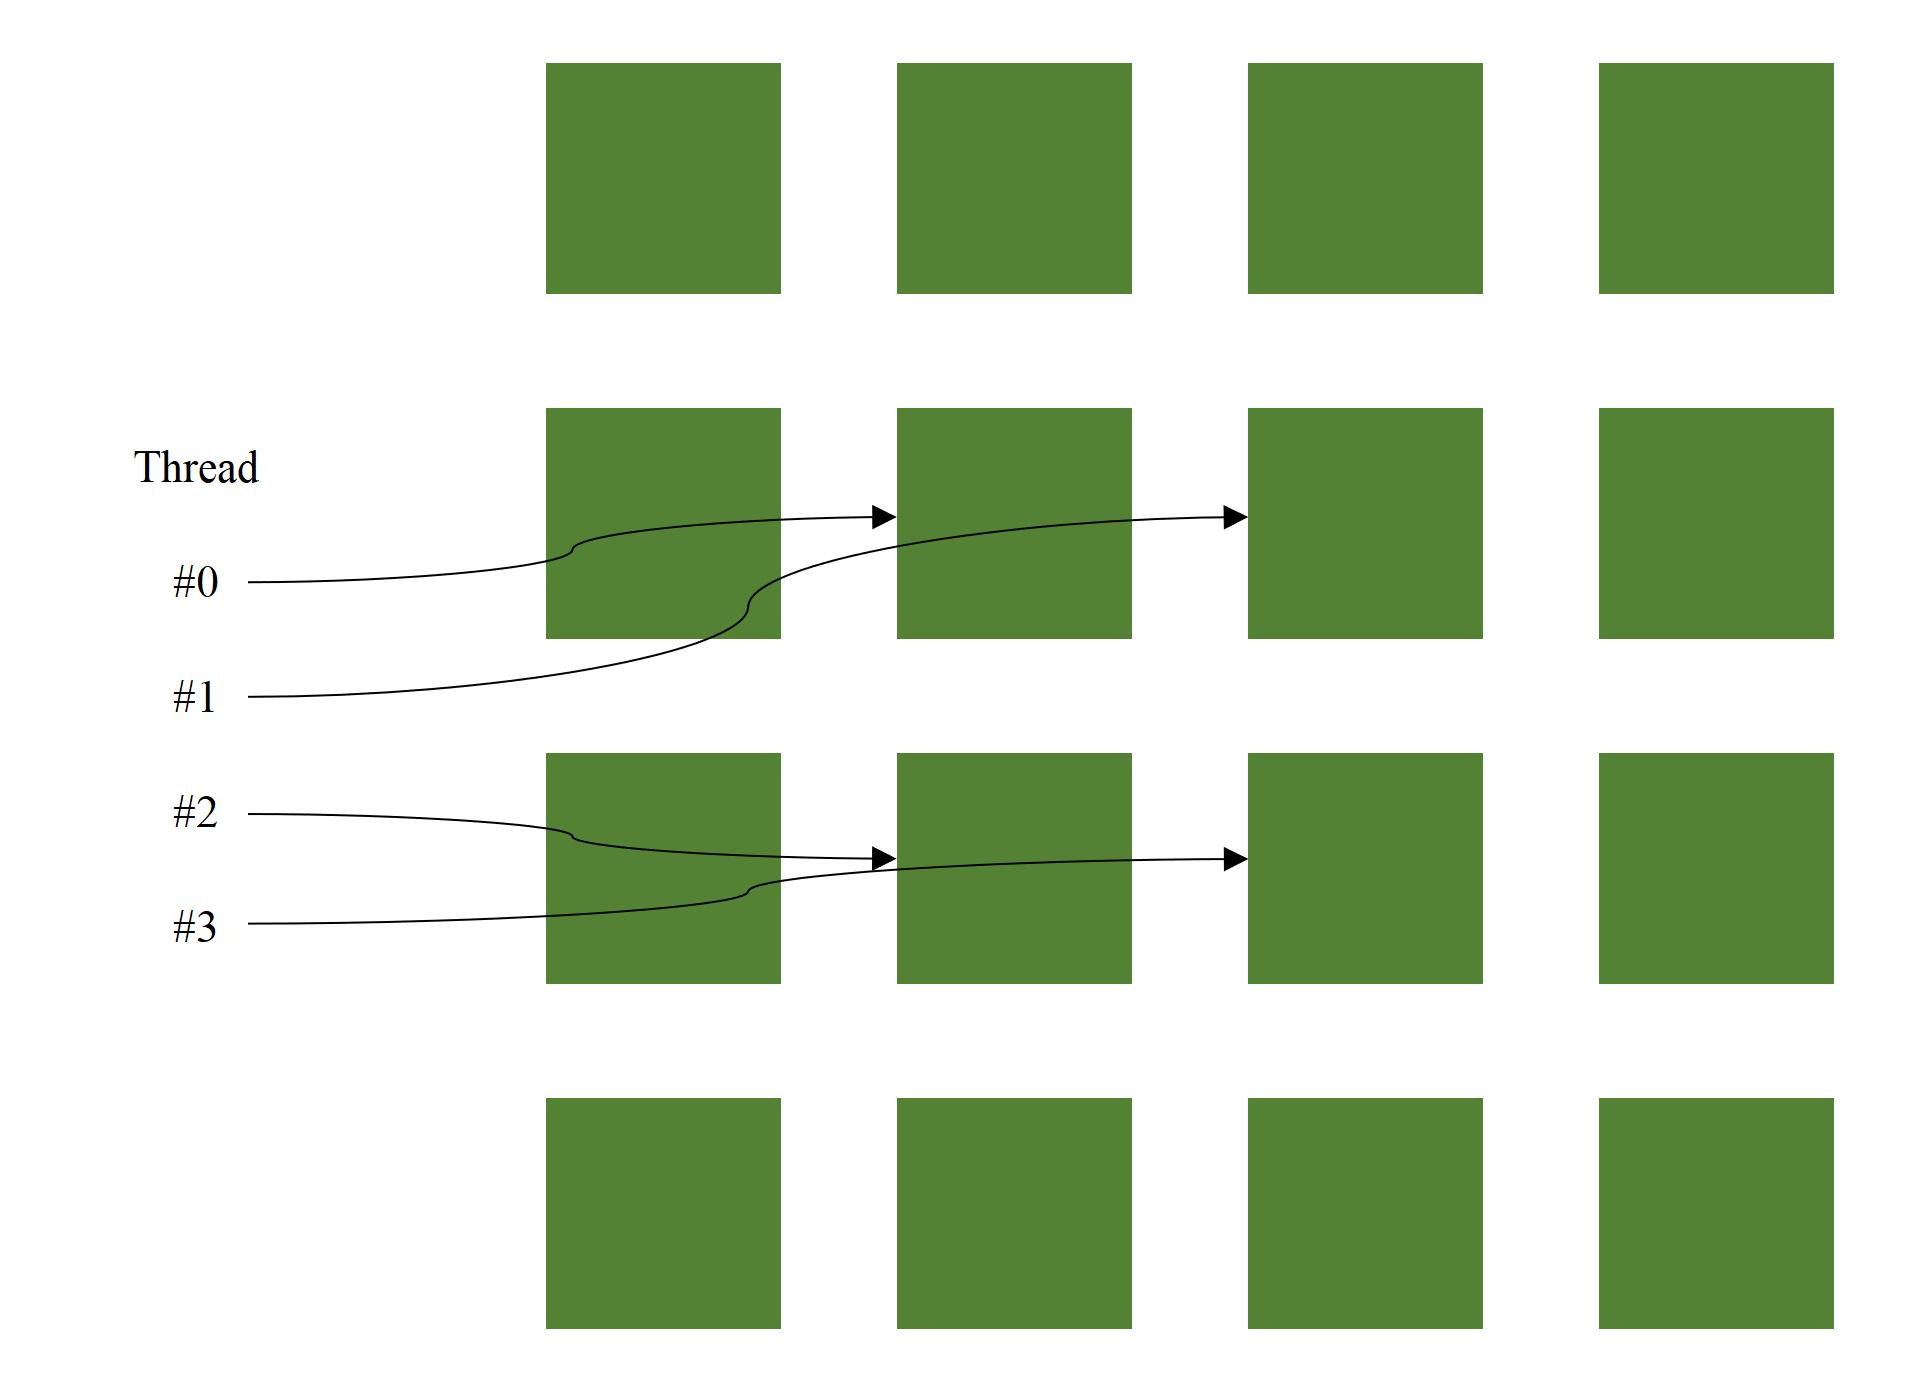
\includegraphics[width=7.5cm]{figures/TextureM.jpg}
	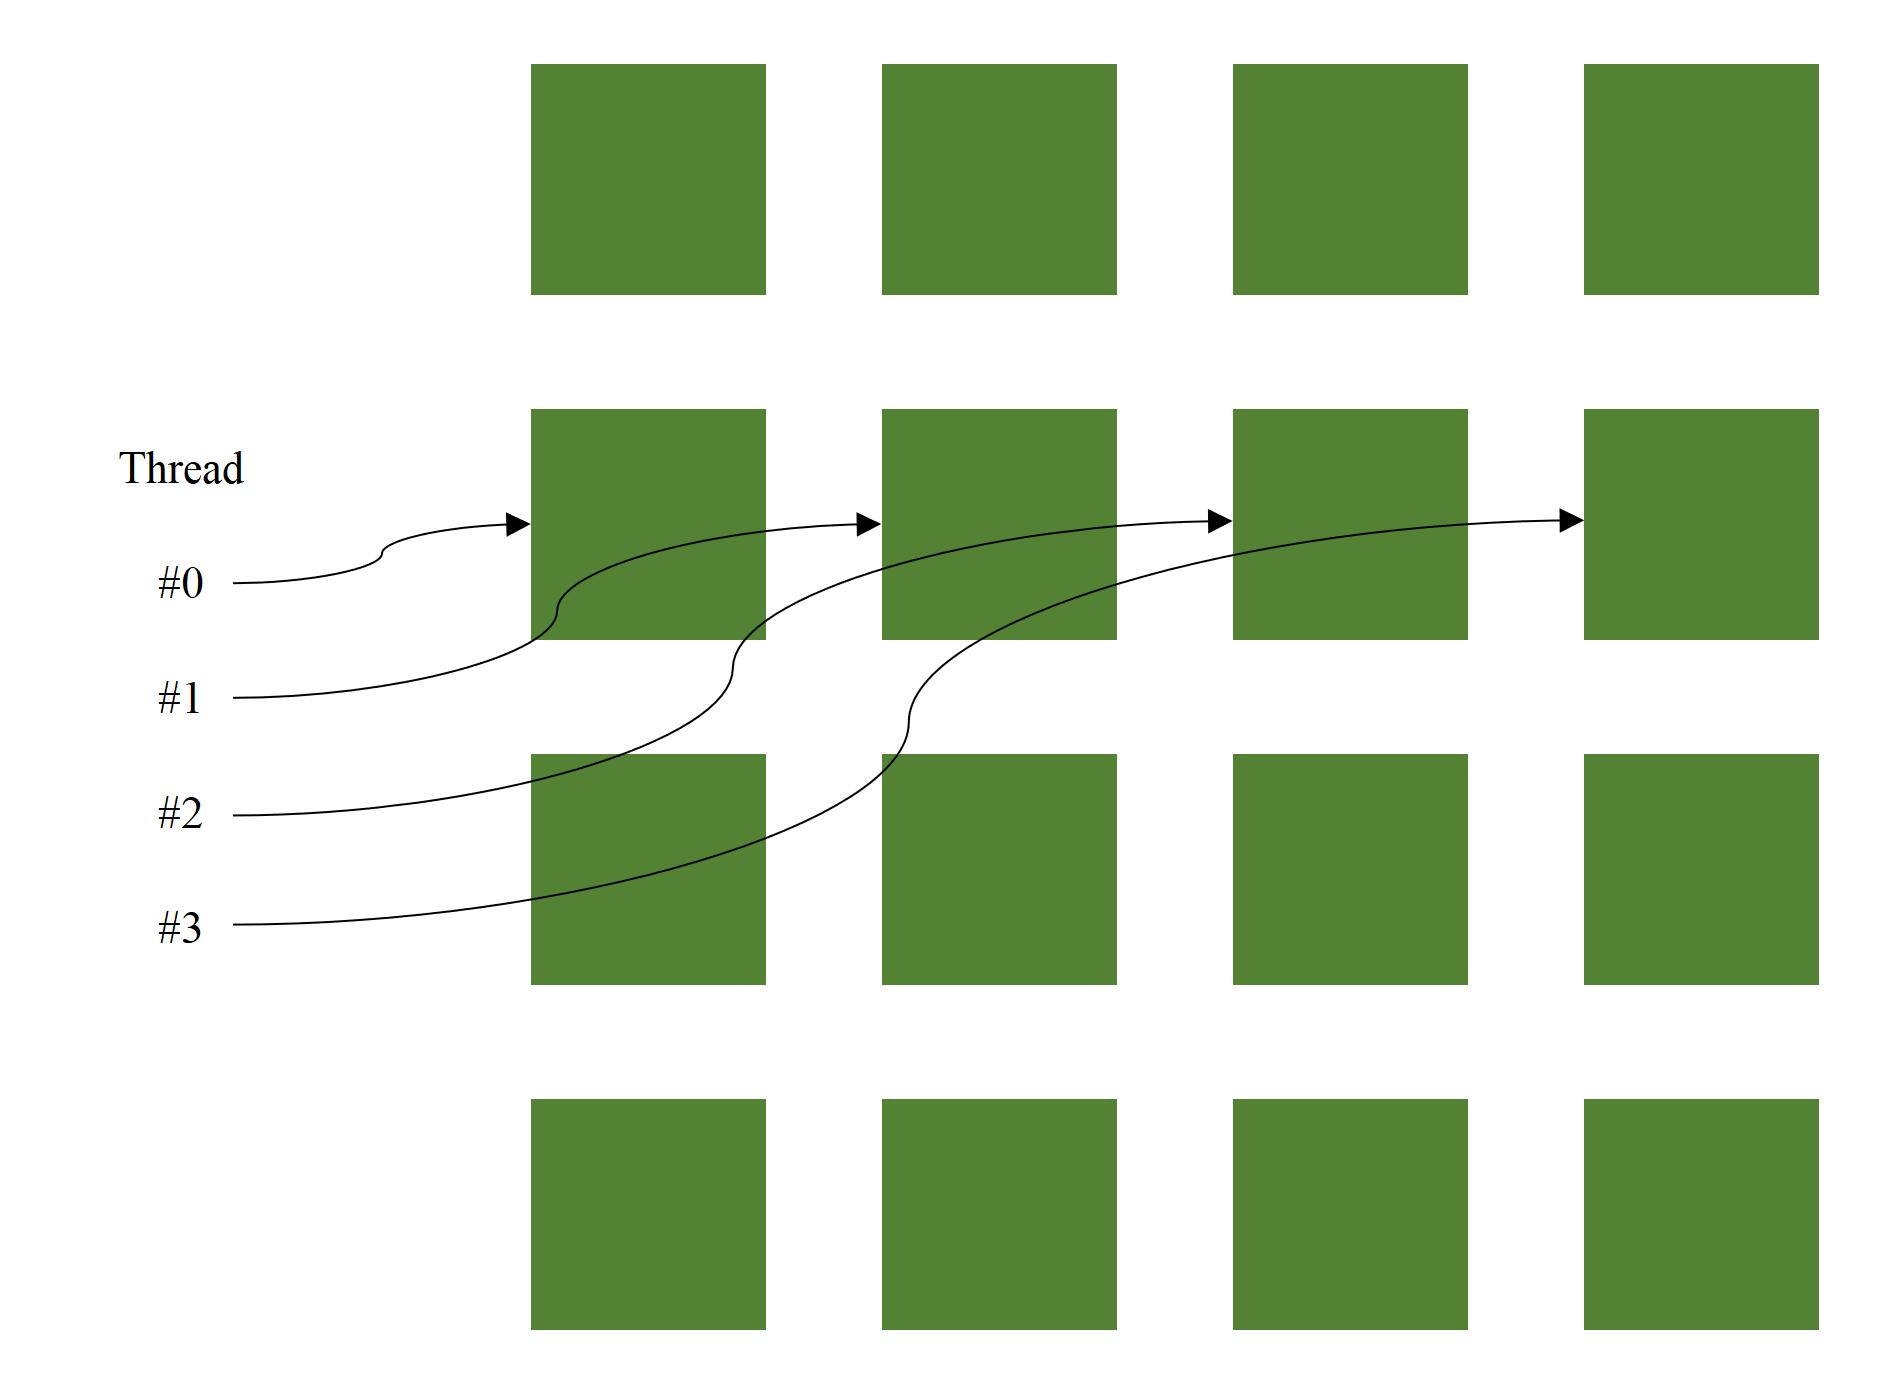
\includegraphics[width=7.5cm]{figures/GlobalM.jpg}
	\renewcommand{\thefigure}{\arabic{section}-\arabic{figure} }
	\renewcommand{\figurename}{图}
	\caption{纹理内存和其余存储系统}
	\addtocounter{figure}{-1}
	\renewcommand{\thefigure}{\arabic{section}-\arabic{figure} }
	\renewcommand{\figurename}{Figure}
	\caption{Texture memory and other memory system}
	\label{Fig.TextureAndGlobal}
\end{figure}

\subsubsection{伏特/图灵架构新硬件}     
\subparagraph{伏特/图灵架构新硬件}
\par 图\ref{Fig.VoltaPascal}展示了伏特/图灵架构(Volta/Turing)与帕斯卡架构(Pascal)在流多处理器单元层面的异同,左侧为伏特/图灵架构、右侧为帕斯卡架构。
\par 在调度方面,指令缓存、线程束调度器与寄存器并无太大差别,而指令分发器(Dispatch Unit)由帕斯卡架构中的每SM两个变为每SM一个,这是因为在处理分支时,如上文提到的在伏特架构以前为了减少线程束内部线程分化带来的性能下降,指令以十六个线程进行分发,故存在两个指令分发器;而后则采用CBU单元处理分支指令,故仅存在一个指令分发器。
\par 在运算单元部分,帕斯卡架构简单的分为计算单元(Core)、访存单元(LD/ST, Load/Store)和特殊功能单元(SFU, Special Function Unit)三个部分,其中计算单元统一为单精度浮点计算单元,访存单元负责一组流处理器依赖数据的请求和结果的写回,特殊功能单元则负责逻辑判断、分支等操作。在新架构中,计算单元根据精度被分为双精度浮点计算单元(FP64)、单精度浮点计算单元(FP32)、整数计算单元(INT)以及最新加入的张量计算单元(Tensor Core),也是本文的重点。在访存单元和特殊功能单元方面的变化本文并不做详细讨论。在新架构中,L1数据缓存的概念也与共享内存的概念统一了。
\begin{figure}
	\centering
	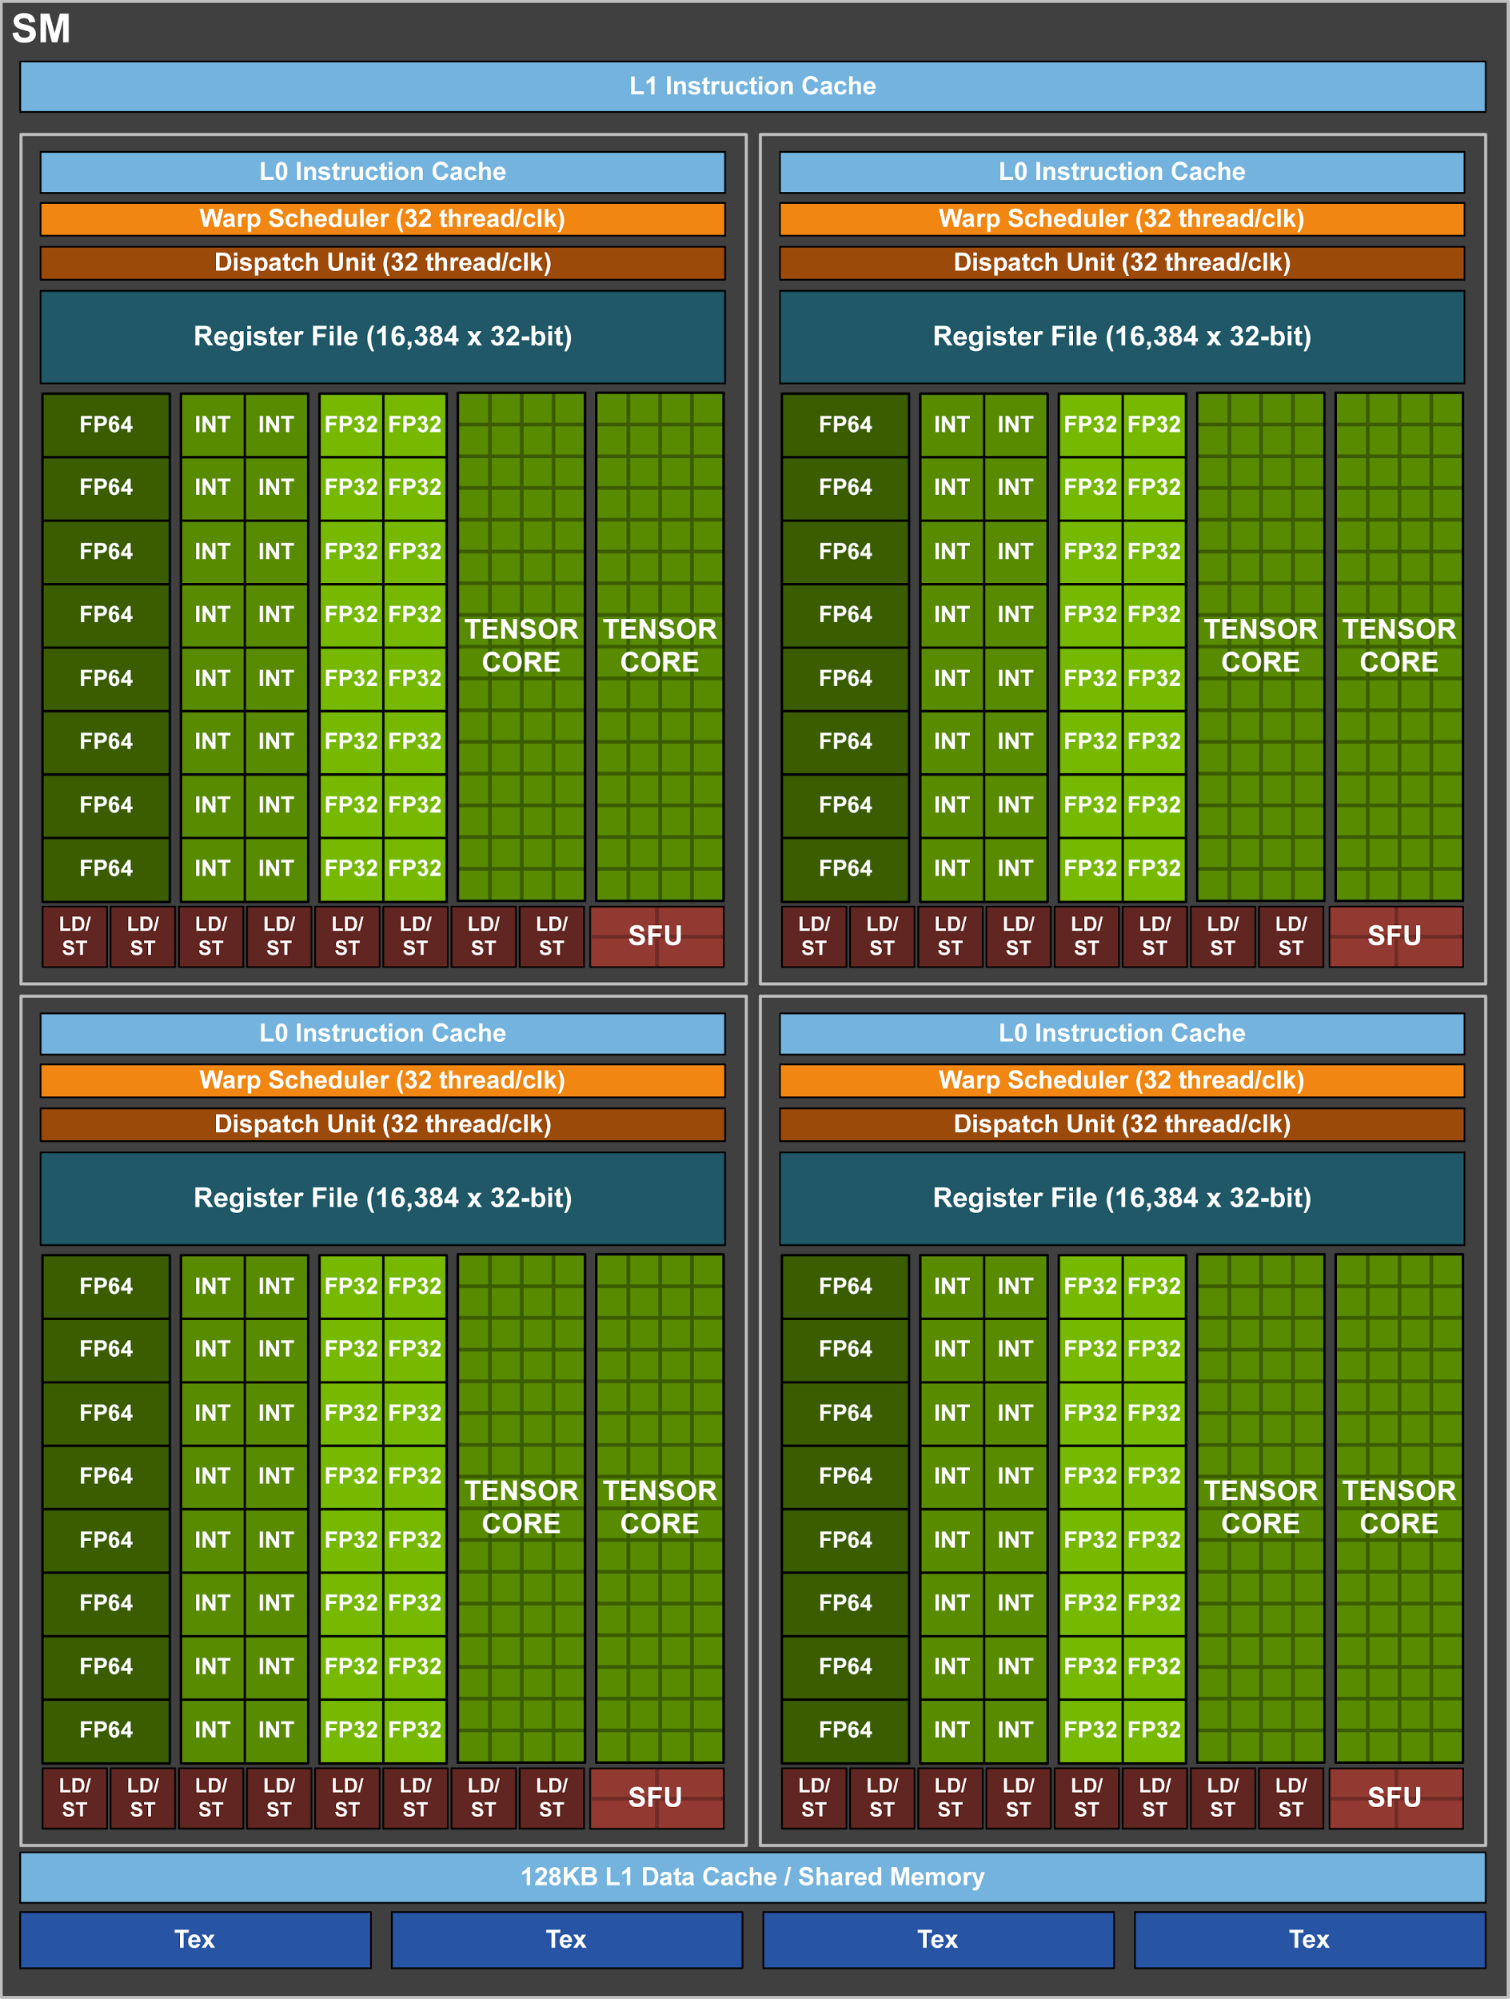
\includegraphics[width=8cm, height=10cm]{figures/VoltaSM.jpg}
	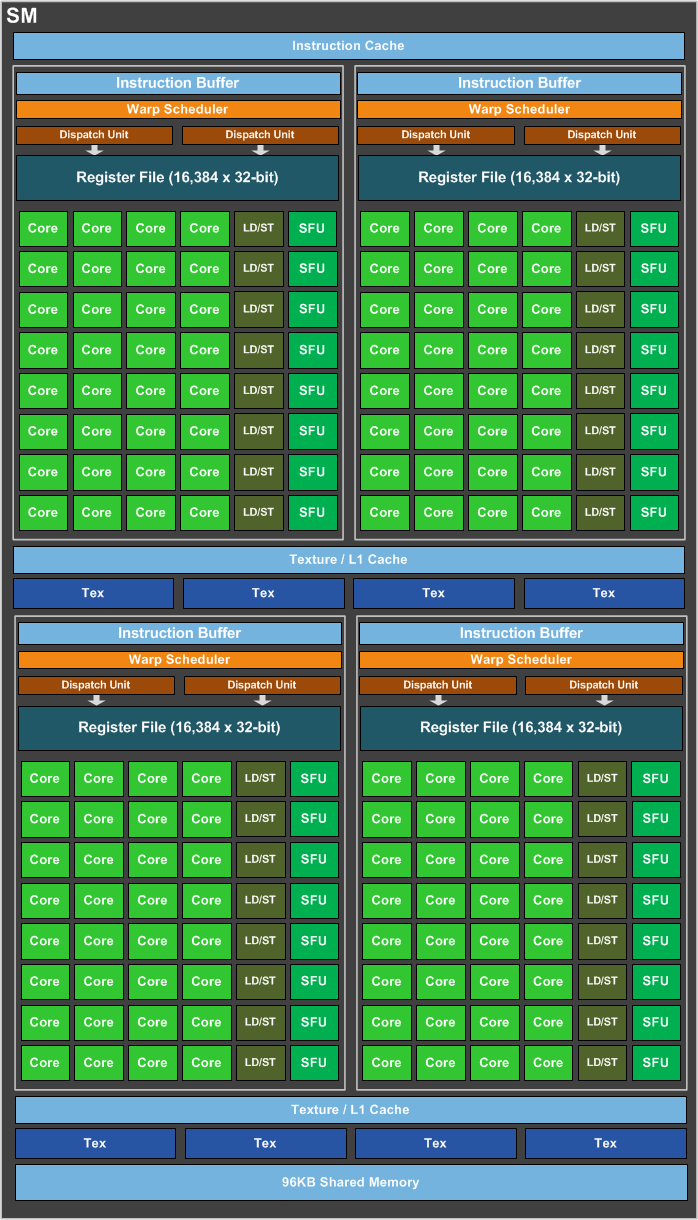
\includegraphics[width=7cm, height=10cm]{figures/PascalSM.jpg}
	\renewcommand{\thefigure}{\arabic{section}-\arabic{figure} }
	\renewcommand{\figurename}{图}
	\caption{伏特架构与帕斯卡架构的流多处理器示意图}
	\addtocounter{figure}{-1}
	\renewcommand{\thefigure}{\arabic{section}-\arabic{figure} }
	\renewcommand{\figurename}{Figure}
	\caption{SM diagram of Volta and Pascal architecture}
	\label{Fig.VoltaPascal}
\end{figure}
\subparagraph{张量核心(Tensor Core)}  
\par 作为本文的重点,张量核心(Tensor Core)将在本文详细介绍。张量核心是一种专为通用矩阵乘法运算(GEMM, GEneral Matrix Multiple)设计的运算单元,对该运算进行了硬件、指令级别的优化,是与老架构最鲜明的区别所在。
\par 在底层的实现中,张量核心以$ 4 \times 4 $的矩阵作为最小的计算单元,被称为$ tile $,任何输入都会被划分为$ tile $进行分块运算,如图\ref{Fig.Tile}所示\cite{CUTLASS}。在伏特架构以前(Volta)的帕斯卡架构(Pascal),一次$ 4 \times 4 $矩阵乘加需要首先调用16次整数点积运算,再将结果累加到乘加矩阵中。而使用张量核心则仅通过一条指令直接完成。根据官方文档给出的描述,这种机制能使伏特架构相比帕斯卡架构再FP16, INT8, INT4精度中分别提供8倍、16倍、32倍的吞吐量提升。实际测试中,Tesla V100再FP16精度下的$ m=2048, k=2048, n = 2048 $规模的矩阵乘加中比Tesla P100块9.3倍\cite{VOLTAWHITEPAPER},这也是上文提到的官方宣称的9倍。在基于Pascal架构以及之前的架构的GPU上,一次4x4矩阵乘法需要调用16次向量点积加和运算,在有idp4a指令支持的GPU上在16个周期内运算出乘积矩阵,若没有指令支持则需要64个周期,而运算得出的乘积矩阵还需要累加;而张量则在更少的周期内完成乘积和加和的运算,具体周期数由hmma指令的操作数决定,对于被分割为$ m=8,n=8,k=4 $的子矩阵的运算,张量核心仅需要八个周期完成所有乘积和加和运算\cite{HMMA}。本节将在各种规模、精度、形状的情况下考察张量实际能够带来的性能提升并探究相应原因。
\par 值得注意的是,在流处理器单元中,张量核心是与其他运算单元包括浮点单元、整数单元共用调度器,调度器每个时钟向分支单元、张量核心阵列、数学分派单元或访存单元发出一个线程束调度指令,这就表明一个周期内硬件不能同时执行张量核心负责的的混合矩阵运算和其他运算,单一周期只能执行单一类型的运算\cite{AMPEREPOR}。张量核心有一定程度的可编程性,但是4x4矩阵仍然是操作的最小单元,在LLVM IR的级别观察其指令仍是如此。尽管被描述为最小4x4为单元的矩阵的混合运算,但实际上张量核心进行的运算总是使用16x16矩阵,并且跨两个Tensor Core进行处理\cite{TENSORCORE},这与其最小调度单元为线程束,也就是32个线程有关。
\begin{figure}
	\centering
	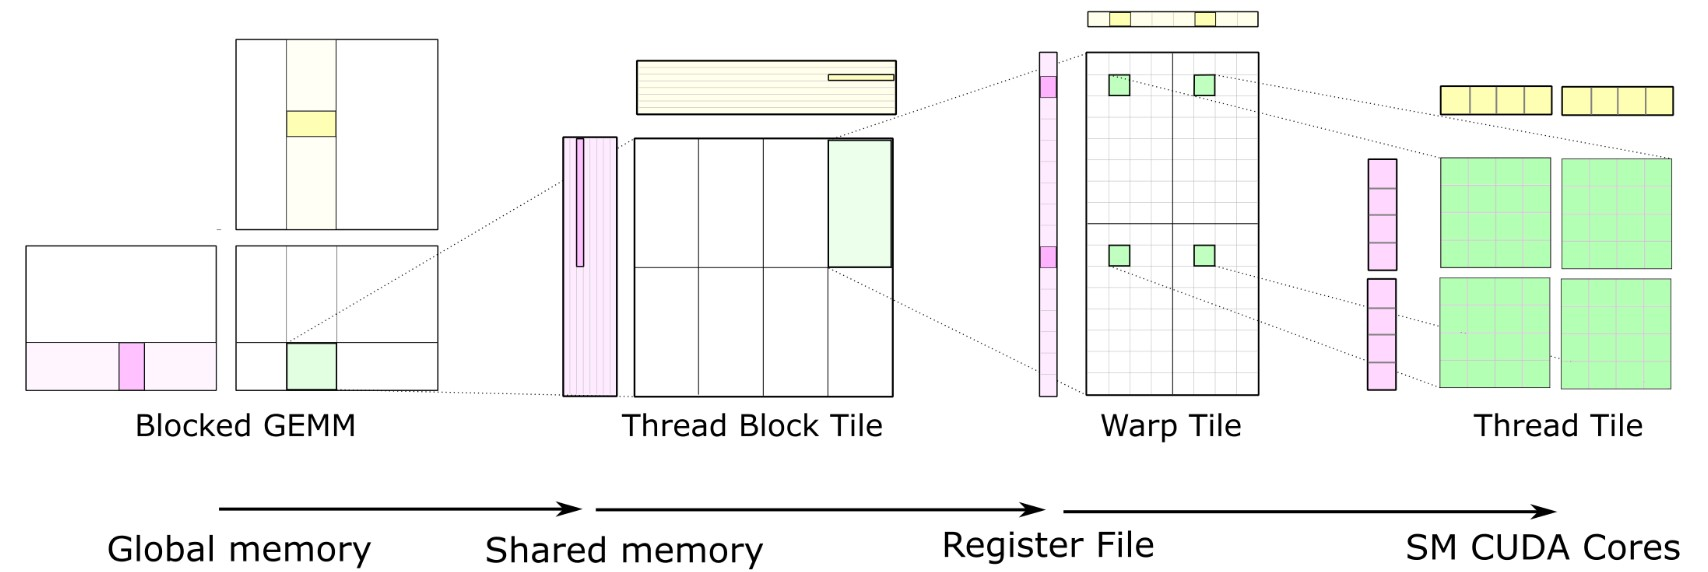
\includegraphics[width=15cm]{figures/Tile.jpg}
	\renewcommand{\thefigure}{\arabic{section}-\arabic{figure} }
	\renewcommand{\figurename}{图}
	\caption{使用张量核心进行通用矩阵乘法计算的层级\cite{CUTLASS}}
	\addtocounter{figure}{-1}
	\renewcommand{\thefigure}{\arabic{section}-\arabic{figure} }
	\renewcommand{\figurename}{Figure}
	\caption{Hierarchy of GEMM using Tensor Core}
	\label{Fig.Tile}
\end{figure}

\subsubsection{线程组织形式与调度方式}
\subparagraph{线程组织形式}
\par 本节将介绍GPU上任务的调用机制。根据弗林分类法\cite{FLYNN},计算机系统可以分为SIMD, MIMD, SISD, MISD等类型。目前多核心CPU系统就是MIMD系统,而NVIDIA的GPU系统被称为SIMT(Single Instruction Multiple Thread)即单指令多线程,与SIMD(Single Instruction Multiple Data)即单指令多数据不同;在这种模型中,一种指令并非仅仅代表一个固定的功能,,而是代表这一指令使用的流水线类别,即指令的类型,线程需要执行的具体操作需要编写相关内核代码。所以,在SIMT模型中,内核程序读入统一的数据,程序代码根据需要进行不同操作;实际调度时不同操作通过重复指令流按顺序发射,只不过运算单元会屏蔽无关线程。
\par 在GPU程序中,32个线程被组织为一个线程束(warp),作为基本的调度单元,拥有各自的物理寄存器。也就是说线程束中的32个线程一般情况下会执行相同的指令流访问不同的数据,即SIMD模式。且线程束目前仍然作为同步的最小粒度,即线程束和线程束可以保证同步,而线程束内部的线程无法保证同步。在下一代安培架构(Ampere)中则将引入$ Arrive-Wait $模式以实现线程级同步,以提高GPU程序的灵活性。
\par 若干个线程束被组织为一个线程块(block),线程块之间通过共享内存进行数据交换,线程块中的线程束可以通过$ \_\_syncthread() $进行同步。在下一代架构中将添加线程束组的层级(warp group),由四个线程束组成,然而该层级仅为大规模通用矩阵乘法指令所用,这里不做讨论。
\par 若干个线程块被组织为一个线程网格(grid),线程网格可被看作一个分配给GPU的任务,故线程网格的虚拟内存空间是相互独立的。
\par 表\ref{table-粒度}详细说明了GPU中不同粒度的线程的组织形式以及相应调度者。
\begin{table}
	\centering
	\renewcommand{\thetable}{\arabic{section}-\arabic{table} }
	\renewcommand{\tablename}{表}
	\caption{线程组织形式}
	\addtocounter{table}{-1}
	\renewcommand{\thetable}{\arabic{section}-\arabic{table} }
	\renewcommand{\tablename}{Table}
	\caption{Type of organizing threads}
	\begin{tabular}{ccc}
		\toprule
		粒度	&	调度者	& 	分配给 \\
		\midrule
		warp		&	线程束调度器	&	流处理器(Stream Processor)\\
		block(CTA)	&	TPC调度器(MPC, M-Pipe Controller)		  &		流多处理器(Stream Multi-processor)\\
		grid		&	GPC调度器(GPM, Graphics Pipe Manager)		  &		TPC(Texture Processing Cluster)$ * $\\
		kernel		&	CPU, PCIe			&		GPC(Graphics Processing Cluster)	\\	
		\bottomrule
	\end{tabular} \label{table-粒度}\\
	
	$ * $ 在本世代图灵架构及以前,TPC与SM可以等价,因为一个TPC上仅包含一个SM,然而自下一代安培架构开始,一个TPC中将会有若干个SM。虽然本文研究的图灵架构的硬件在逻辑上SM与TPC等价,但在硬件上还是会做区分,故在表中详细写出\cite{BLOCKDIAG}。
\end{table}
\subparagraph{调度方式}
\par 以上内容介绍了GPU线程的组织形式,这里将介绍GPU线程的调用方式,在介绍调用方式之前,需要先明确GPU与CPU的硬件上的差别,主要有如下几点。
\begin{itemize}
	\item GPU中存在大量的物理寄存器,达几十~几百KB,且都能在1个时钟周期内访问,而CPU中物理寄存器资源极为有限。故在进行上下文切换时,GPU只需更改寄存器文件指针来切换,而CPU需要使用堆栈保存上下文。
	\item CPU仅仅支持数十个硬件线程,而GPU则支持数千个硬件线程。在GPU上开启过少的硬件线程会极大降低硬件使用率,进而导致性能降低。具体开启线程数量取决于硬件SM最大并发线程数、最大并发线程束数和最大并发块数等。表\ref{table-占用率}显示了在不同计算能力上开启不同数量的线程时设备的利用率以及所能开启包含该数量线程的线程块的数量。\\
	\begin{table}
		\centering
		\renewcommand{\thetable}{\arabic{section}-\arabic{table} }
		\renewcommand{\tablename}{表}
		\caption{可分配线程数与占用率的关系}
		\addtocounter{table}{-1}
		\renewcommand{\thetable}{\arabic{section}-\arabic{table} }
		\renewcommand{\tablename}{Table}
		\caption{Available thread number and corresponding occupancy rate}
		\begin{tabular}{cccccc}
			\toprule
			&	1.0	&1.2	&2.0	&2.1	&3.0 \\
			\midrule
			64	&	67\%, 8		&	50\%, 8		&	33\%, 8		&	33\%, 8		&	50\%, 16	\\
			96	&	100\%, 8	&	75\%, 8		&	50\%, 8		&	50\%, 8		&	75\%, 12	\\
			128	&	100\%, 6	&	100\%, 8	&	67\%, 8		&	67\%, 8		&	100\%, 10	\\
			256	&	100\%, 3	&	100\%, 4	&	100\%, 6	&	100\%, 6	&	100\%, 8	\\
			512	&	67\%, 1		&	100\%, 2	&	100\%, 2	&	100\%, 3	&	100\%, 4	\\
			1024&	N/A, N/A	&	N/A, 1		&	67\%, 1		&	67\%, 1		&	100\%, 2	\\
			
			\bottomrule
		\end{tabular} \label{table-占用率}
	\end{table}
	可见,随着计算能力的增长,一个流多处理器上所能容纳的线程束数量越多。在充分利用寄存器文件和共享内存(L1缓存)的情况下开启线程数越多,设备利用率越高。然而过多的线程会导致资源紧缺,在实际使用中应当根据硬件参数,问题规模做出调整。
	\item 发生分支时,CPU采用分支预测-预测错误则清空流水线的机制进行,而GPU则引入了线程束分化的概念,这一概念将在下文详细介绍。
\end{itemize}
\par GPU程序首先由内核(kernel)开始,一个内核代表一个需要在GPU上运行的程序,由CPU管理、分配给GPU上的图形处理簇(GPC)。一个大任务会被拆分为若干小任务,这些小任务被抽象为线程网格(grid)由图形处理簇上的调度器分配给纹理处理簇(TPC)。在纹理处理簇上的调度器将以线程块(block)为单位将线程分配给流多处理器单元(SM)。最后,具体的运算任务将由流多处理器单元内部的线程束调度器分配给不同流处理器(SP)。
\par 在调度时,线程束作为最小的调度单元在一般情况下将会运行同一指令流,这一情况在发生分支时会有不同。线程束被分发到分支指令时,若线程束内部线程发生分化(即一部分执行分支,一部分不执行分支),则两个分支都会被执行,分支结束时只有执行了正确分支目标的线程会被置未激活状态,执行了错误分支目标的线程被设置为未激活状态。由于线程束调度器每次只能为一个线程束取到一条指令,这意味着线程束内部发生线程分化时,未激活状态的线程会被阻塞,导致利用率、性能下降。自麦克斯韦架构开始,为了尽可能减小线程束内部线程分化对性能造成的影响,指令是以半个线程束即十六个线程进行分发的。之后,GPU引入了CBU单元(Convergence Barrier Unit)以保持通过同一分支的线程被组织在一起的方式尽可能减少分支带来的性能下降\cite{THREADS}。在实际编程中,GPU提供非常细致的线程、线程块、线程网格ID,故根据这些ID控制分支使得线程束内部线程分化尽可能减少是可行的\cite{DIVER}。
\par 最后将介绍GPU中的流以及相应的锁页内存的概念。GPU中的流可以被看做一个GPU操作队列,该队列中的操作将会按顺序执行。这一特点使得在实际编写程序的过程中可以通过调整不同操作的顺序,如访存、密集计算、写回等来隐藏数据依赖和控制依赖带来的延迟\cite{STREAM},通过异步操作(ASYNC)提高任务级并行度。CUDA流需要在支持设备重叠的GPU上运行,设备重叠使得GPU能够在执行一个核函数时在设备和主机间进行数据交互。而为了支持流,所有涉及流的内存需要在锁页内存上进行分配。锁页内存正如其字面含义,是分配在显存上、不允许被移动或被换页到磁盘上的设备内存。其好处是允许GPU上的DMA控制器绕过CPU直接请求主机传输数据,在延迟更低的基础上支持设备重叠\cite{PAGELOCK}。若不使用锁页内存,DMA控制器在定位内存页面时会造成困难。本文的部分实验中使用了流这一特性,将在具体实验章节详细介绍。

\subsection{NVIDIA GPU相关软件}
\par 本节将自顶向下介绍NVIDIA GPU硬件对应的不同层级的编程平台及相关工具。
\subsubsection{机器学习框架(Tensor Flow)}
\par 近年来机器学习尤其是深度学习发展迅猛,各种方便程序员搭建模型的框架层出不穷。考虑到机器学习应用的计算量要求日益攀升,这些框架都陆续推出了基于GPU的版本。为方便程序员搭建模型,框架本身对硬件的操作进行了抽象。然而,正是因为这一层抽象,忽略了许多硬件层面的细节,使得框架无法完全利用硬件的性能。这也导致了许多用户反映在实际应用中,新架构的性能提升并没有官方给出的文档数值、硬件参数(包括流处理器、纹理/光栅单元)、甚至价格上涨幅度那么多。本文将挑选目前非常流行的Tensor Flow框架作为最上层应用的研究载体,考察如何根据硬件特性对Tensor Flow级别的源码以及Tensor Flow本身的源码(基于C/C++)进行优化以达到更快的速度、更高的吞吐量。为达到这一目的,需要对Tensor Flow框架从源码重新编译,具体步骤此处不再赘述\cite{TFBUILD}。
\subsubsection{CUDA}
\par CUDA(Compute Unified Device Architecture)是由英伟达(NVIDIA)针对图形处理单元开发的并行计算平台及对应的编程模型。在编写CUDA程序时,程序员通过在一些较为热门的编程语言包括C/C++、Python、Matlab、Fortran中以关键字的形式加入扩展来描述并行行为\cite{CUDAZONE}。本文选用C/C++进行CUDA的扩展,基础的核函数编写、存储系统调用\cite{EVENEASIER}此处不再说明。
\par 在本文中的实验进行时,CUDA SDK最新版本为10.0,主要在CUDA SDK 9.2的基础上对图灵架构进行了支持;对更多分割尺寸的通用矩阵乘法运算进行了支持\cite{10.0PATCH};以及对多GPU、不同操作系统、兼容性等方面进行了更好的支持。而CUDA SDK 9.2相对于CUDA SDK 9.0则更新了对伏特架构以及对应张量核心(Tensor Core)的支持,属于一次较大的更新\cite{9.2PATCH}。在文章撰写之际,NVIDIA推出了CUDA SDK 10.1,在CUDA SDK 10.0的基础上更新了轻量级矩阵乘法库;更新了对应的构建、测试工具等\cite{10.1PATCH}。CUDA SDK 10.1的更新对于本文的实验结果并无决定性的影响,故本文仍然采用CUDA SDK 10.0进行实验。
\par CUDA程序经过一系列工具如nvcc等被编译为中间代码(PTX),再从中间代码编译为能直接运行于目标硬件的硬件代码(SASS)。
\subsubsection{硬件代码(SASS)与中间代码(PTX)}
\par 中间代码(PTX, Parallel Thread eXecution)\cite{PTX}是一种并行线程执行虚拟机代码(IR),在实际运行时,该中间代码会被编译为硬件代码(SASS)。本实验中为了详细观察硬件层面的操作,将在编译上层应用程序时添加$ --keep $保留编译时产生的中间文件。同时,本节将简单介绍中间代码的语法供后文使用。
\par 中间代码中由两种语句:Directive Statement和Instruction Statement,前者起到声明作用,后者则是具体运算动作,起到声明作用的语句在此不再赘述,详细考察具体运算动作的指令,以本文中的重点:线程束级矩阵乘加指令(wmma, warp-level matrix multiply Accumulate),也就是张量核心使用的指令为例,如图\ref{Fig.Inst}所示。中间代码主要分三个部分:指令、具体操作和操作数与传统的SIMD模型中的指令、操作数不同,在SIMD模型中,其“多线程”的特点正是对应了中间代码中的具体操作这一部分。在具体操作这一部分中,中间代码会指明存/取、是否同步、操作数数据分布(行/列主元素)、数据精度等项目。图\ref{Fig.ActualInst}是一段具体的涉及wmma指令的中间代码,代码中操作数形状、数据类型等将在实验中具体介绍。
\par 硬件代码(SASS)与中间代码(PTX)类似,分为指令、具体操作和操作数三个部分,其区别是硬件代码会开放涉及浮点数存储方式、分支预测操作等底层的、直接对硬件进行的操作,本文中不再详细介绍,仅会在涉及张量核心的实验中提到对应中间代码中wmma指令的硬件代码中的hmma指令。
\begin{figure}
	\centering
	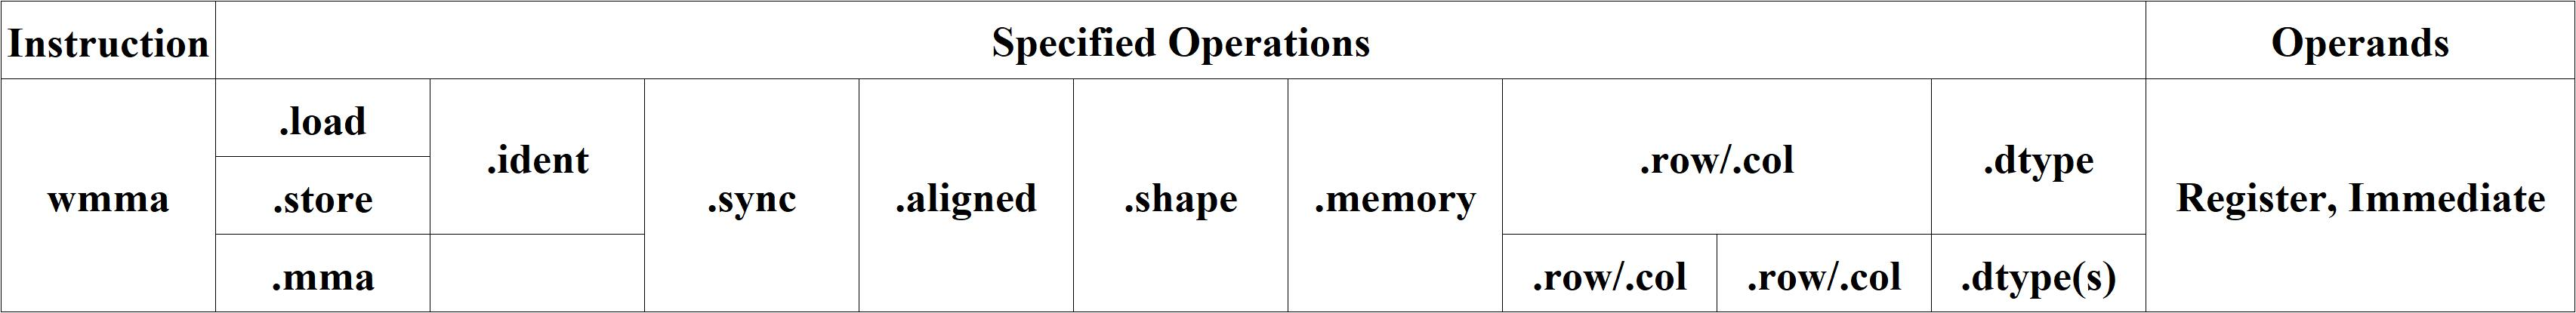
\includegraphics[width=15cm]{figures/Inst.jpg}
	\renewcommand{\thefigure}{\arabic{section}-\arabic{figure} }
	\renewcommand{\figurename}{图}
	\caption{中间代码(PTX)格式示例} 
	\addtocounter{figure}{-1}
	\renewcommand{\thefigure}{\arabic{section}-\arabic{figure} }
	\renewcommand{\figurename}{Figure}
	\caption{An example of PTX code}
	\label{Fig.Inst}
\end{figure}
\begin{figure}
	\centering
	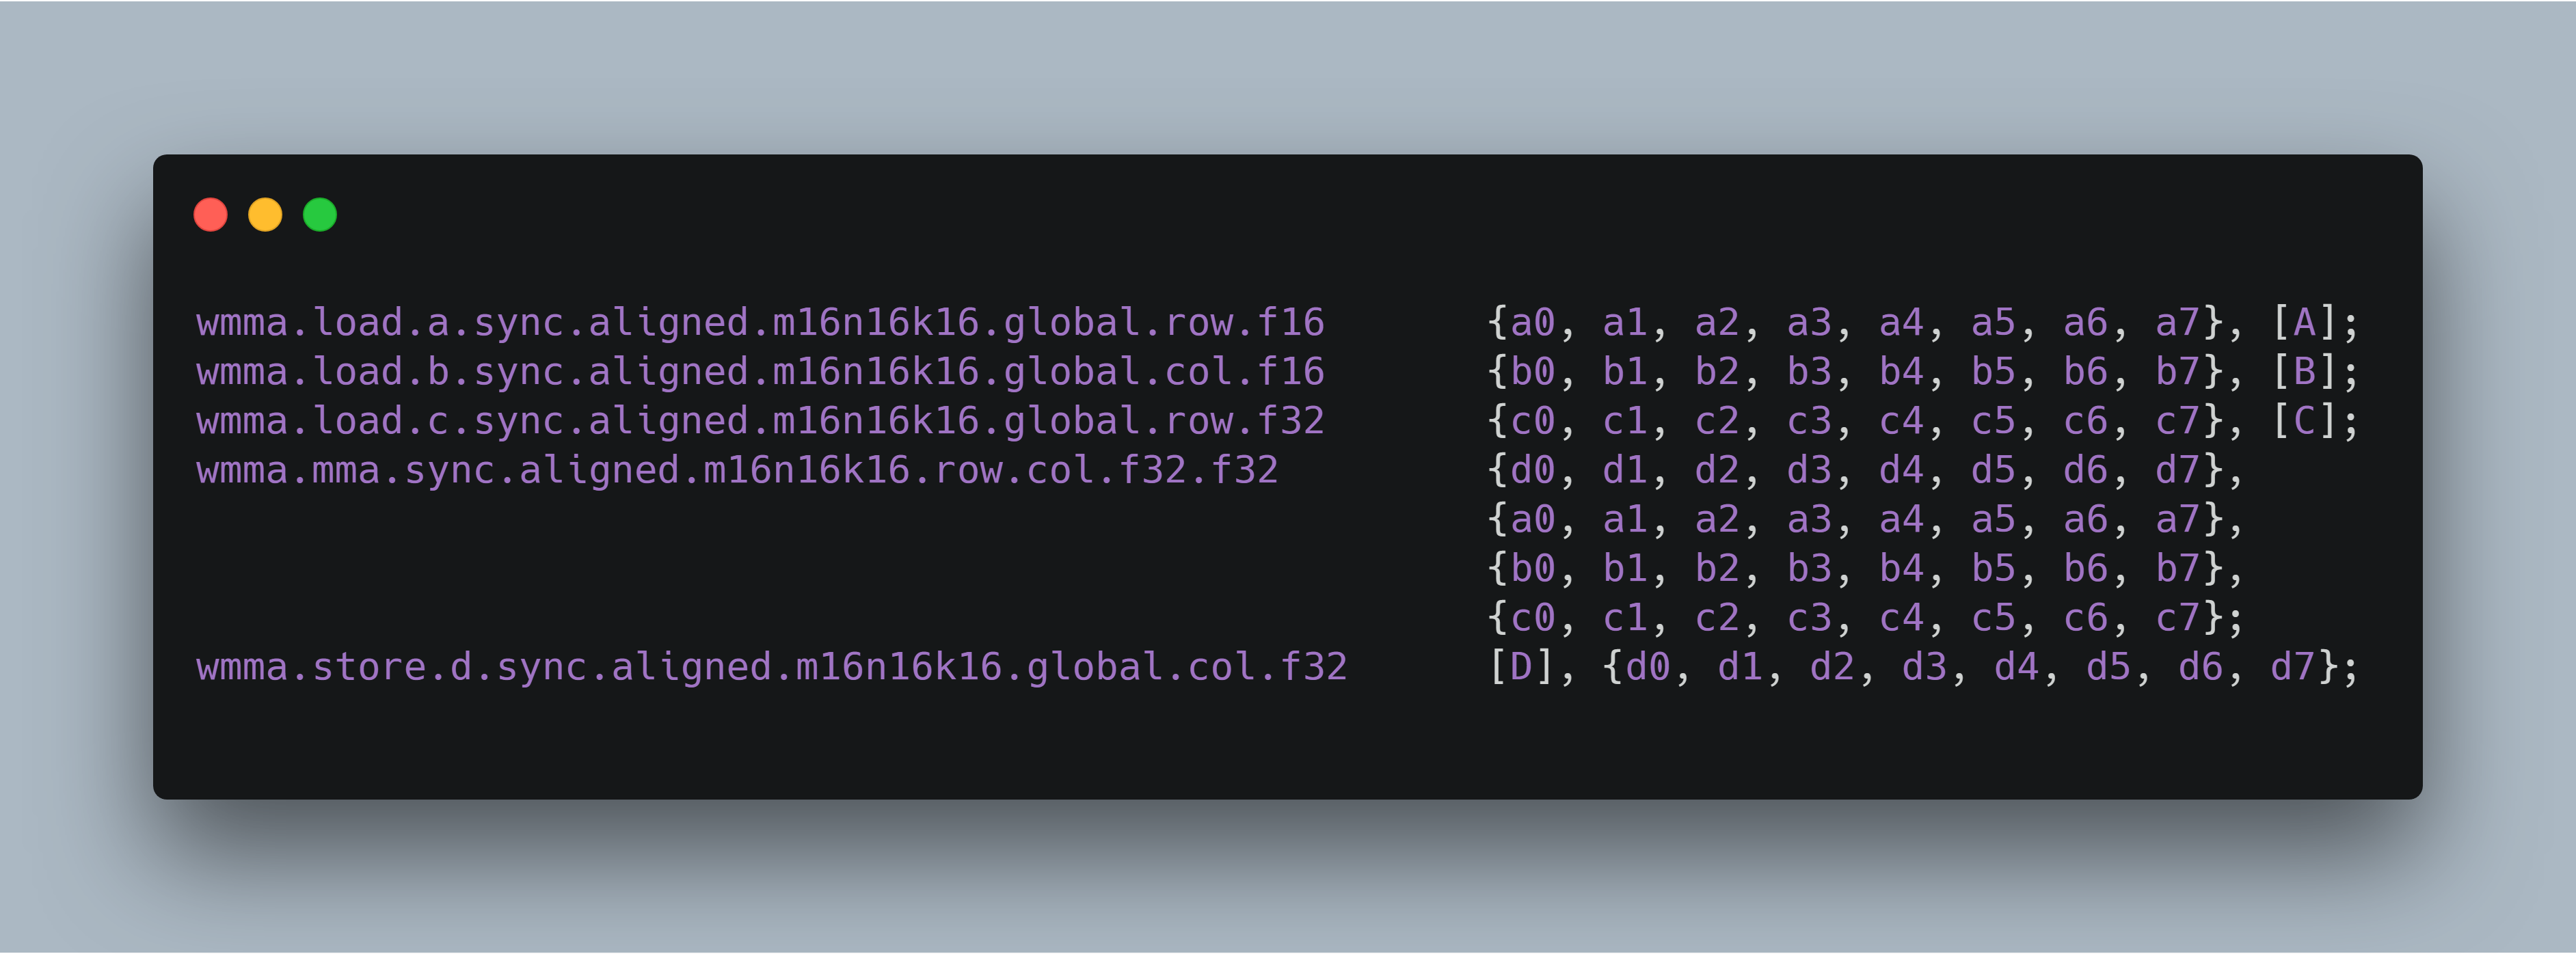
\includegraphics[width=15cm]{figures/ActualInst.jpg}
	\renewcommand{\thefigure}{\arabic{section}-\arabic{figure} }
	\renewcommand{\figurename}{图}
	\caption{一段具体的中间代码(PTX)}
	\addtocounter{figure}{-1}
	\renewcommand{\thefigure}{\arabic{section}-\arabic{figure} }
	\renewcommand{\figurename}{Figure}
	\caption{Part of actual PTX code}
	\label{Fig.ActualInst}
\end{figure}
\subsection{神经网络推理工具 TensorRT}
\par 在实际的机器学习应用中,模型的训练只是第一步,在模型完成训练后需要对模型进行部署。当模型构建完毕,实际部署到目标机器、芯片、平台上并发挥作用是,推理就成为了主要工作。与训练的过程和目的不一样,推理首先没有了训练过程中的反向迭代,同时对于吞吐率、延迟、功耗等有着更高的要求;且现有框架在实际部署时因其复杂度高,对部署造成了很大困难,TensorRT由此而生。
\par TensorRT是一个高性能深度学习推理的平台,包含深度学习推理优化器和运行时应用来提供低延迟、高吞吐量的深度学习推理。本节将考察TensorRT相对于传统神经网络推理的加速性能\cite{TENSORRT}。因TensorRT原生支持Tensor Flow,这就意味着可以直接使用TensorRT自带的模型导入器对训练好的模型进行导入,故本文通过这种方法来考察TensorRT的实际提升。
\par 在实际使用TensorRT之前,将先对TensorRT的优化以及部署流程进行介绍。首先需要明确的是,TensorRT作为一个GPU Inference Engine(GIE),它是在项目部署阶段发挥作用的。TensorRT的部署分为两个部分:优化训练好的模型并生成计算流图和使用TensorRT Runtime部署计算流图。其最重要的便是优化过程,如下图\ref{Fig.TensorRT}所示\cite{TENSORRTDOC}。
\begin{figure}
	\centering
	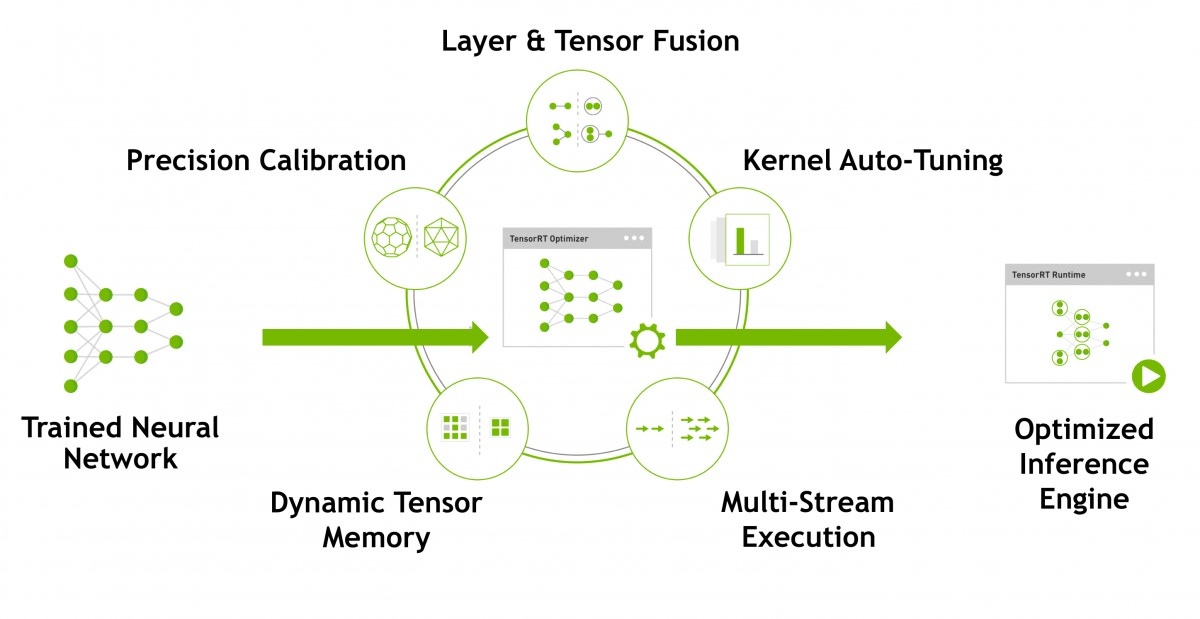
\includegraphics[width=15cm]{figures/TensorRT.jpg}
	\renewcommand{\thefigure}{\arabic{section}-\arabic{figure} }
	\renewcommand{\figurename}{图}
	\caption{TensorRT中的模块\cite{TENSORRT}}
	\addtocounter{figure}{-1}
	\renewcommand{\thefigure}{\arabic{section}-\arabic{figure} }
	\renewcommand{\figurename}{Figure}
	\caption{Modules in TensorRT}
	\label{Fig.TensorRT}
\end{figure}
\par 优化过程的第一部分,也是较为重要的部分便是网络层和张量的合成,这一过程将会在不改变底层计算内容的情况下重构计算图来获得更高效的计算方式。DL框架在进行推理时会执行多个子过程,这些过程都需要GPU Kernel来运行,这就不可避免地带来会更多Kernel Launch,如前文所说,Kernel Launch所带来的上下文切换仍然是很大的开销。TensorRT主要从Kernel纵向融合(如卷积、偏置、激活层的Kernel可以融合为一个Kernel);Kernel横向融合(挖掘输入数据形状相同但权重不同的层,使用一个Kernel而非原来的若干个Kernel提高效率)和消除Concatenation层(通过预分配输出缓存、不同的写入方式来避免转换)。
\par 第二部分,即能鲜明体现新硬件的部分:FP16和INT8精度校准。大部分网络在训练是为了精度,会使用FP32,因此最后输出模型也是基于FP32精度。然而完成训练也就意味着参数达到最优,在推理过程中由于没有反向传播故采用更低的精度能在不牺牲过多准确率的情况下极大提高网络计算吞吐率。
\par 第三部分,动态分配的张量显存能在使用期间减少显存占用率,增加显存复用率,从而避免过度开销以提高推理性能。
\par 最后便是Kernel自动调整和多流执行,TensorRT会针对输入数据大小,filter大小,张量数据分布,batch大小针对目标GPU进行选择和优化,这一部分与传统编译器后端处理,即及其相关优化较为相似。同时TensorRT也会借助CUDA流来提高任务级并行度,这点也在上文提到过。
\par 由于经过TensorRT优化后的模型只能运行于特定硬件平台(TESLA T4, TESLA V100, Jetson系列)\cite{TENSORRTDOC},本文将采用由NVIDIA提供的Jetson TX2开发套件进行TensorRT部分的实验,NVIDIA的Jetson系列是专为嵌入式机器学习应用设计的芯片。在GTC 2019会议中,NVIDIA发布了基于最新技术的Jetson Xavier,然而由于成本原因,本文不使用该硬件。

\subsection{性能评估(Profiling)工具}
\par 为了详细地考察硬件底层的运行机理,实验中采用了若干不同层级的性能评估工具。
\begin{itemize}
	\item Nsight:该工具用于在后台监听CUDA程序的执行流,结合Visual Studio中的工具可以通过可视化的方式直观地观察CPU/GPU调用、上下文切换等信息\cite{NSIGHT}。
	\item nvprof:通过该工具分析某一CUDA程序,可以获得程序执行时的分支效率、访存效率、各API调用占比等信息\cite{NVPROF}。
	\item GPGPU-SIM:该工具支持从中间代码(PTX)层级对CUDA程序的运行进行模拟、仿真,该工具能够提供缓存是否命中、分支是否执行、指令执行周期数等信息\cite{GPGPUSIM}。与GPGPU-SIM搭配的还有NVIDIA内部使用的硬件代码(SASS)层级的仿真工具SMart,该工具能够更为详细地提供指令运行时硬件的各种信息。由于涉及企业机密本文将不详细说明SMart工具的细节。
\end{itemize}
\subsection{基于GPU的机器学习应用}
\par 随着当今机器学习,尤其是深度学习应用中数据量、网络结构复杂度的增长,该类应用对于硬件计算能力的要求也迅速增长。而在这类应用中,有许多密集的计算互相之间是没有数据/控制依赖的,也就是可以并行执行的;比如神经网络前向、反向传播中的权重矩阵计算,这些权重在同一轮计算中不存在耦合性;随机森林(Random Forest)中不同分类器的训练,这一特征可以利用到GPU处理中流这一特征;一系列聚类算法,包括DBSCAN、K-Means等;而图形处理单元(GPU)的设计初衷正是大规模并行计算,也因为GPU的计算能力,深度学习自上世纪末至今迅猛发展,同时GPU的运算性能以及相应的软件的发展也非常迅速。目前,GPU更多代表了通用处理单元(General Purpose)。
\par 当然,GPU上的编程模型与CPU上的模型有较大差别,为了方便程序员搭建模型,目前市面上的许多框架都更新了对GPU的支持。然而,这些框架方便了程序员的程序编写,抽象了底层硬件的细节,比如在CUDA中,线程块、线程束的调度以及相应寄存器文件的分配会对程序性能造成极大影响,然而这些特征都被框架抽象这就导致了硬件性能无法得到完全的发挥。且目前大部分框架都是基于旧的架构和旧SDK编译,没有对新架构与新SDK做出优化。本文的目的也是在于挖掘出新架构的硬件以及对应的新的SDK中的代码翻译、指令执行等部分的特征以及相较老架构和老SDK的变化;根据分析得出的结论修改已有GPU程序的源码,尝试修改选定框架(Tensor Flow)的源码,并给出实际的修改、编程时的建议。
